\begin{savequote}[8cm]
\textit{Es müsse eine Art der Kerntheilung geben, durch welche die im Mutterkern enthaltenen Ahnenplasmen dergestalt auf die Tochterkerne vertheilt werden, dass jedem Tochterkern nur die halbe Zahl derselben zukomme.}

There must be a form of nuclear division in which the ancestral germ plasms contained in the nucleus are distributed to the daughter nuclei in such a way that each of them receives only half the number contained in the original nucleus.
  \qauthor{--- \cite{Weismann1887Ueber}}
\end{savequote}

\chapter{\label{ch:1-intro}Background}

\minitoc


\section{Aims}
Meiosis is a type of cell division in which the number of chromosomes is reduced by half to produce haploid gametes (sperm and egg cells)~\parencite{Ohkura2015Meiosis}. The primary aim of this research was to delineate the gene expression programme of spermatogenesis (during which meiosis occurs). Specifically, to identify which genes are expressed, in which cells, their degree of expression, and relative timing during spermatogenesis. With this atlas of expression data, we additionally aimed to infer the regulatory network controlling these expression patterns, as well as to predict protein function and in doing so identify targets for further characterisation. Finally, we aimed to carry out such characterisation for at least one of these targets.


\section{Motivations}

\subsection{Sexual Reproduction}
Reproduction is a fundamental property of all known life. Of the two empires of life Eukaryotes/Eukarya are able to reproduce sexually, and almost all do. The dominance of this trait has been estimated at roughly 99.9\% \parencite{White1978Modes}, with examples of exceptions being the Bdelloid rotifers - who lost the ability to reproduce sexually 60 Mya, and appear to be evolving by horizontal gene transfer \parencite{Debortoli2016Genetic}. This shared characteristic was likely present in the common ancestor of this empire and hence synapomorphic \parencite{Bernstein2013Evolutionary}. The sexual life cycle consists of an alternating halving of the genetic material/ploidy (by meiosis) to form haploid cells, followed by karyogamy (nuclear fusion). Meiosis (from Ancient Greek, meíōsis, “a lessening”) is a specialised form of cell division, in which genetic material is exchanged between the parental genomes (recombination). Recombination and independent assortment of homologous chromosomes generate genetic diversity and hence enable natural selection and evolution. Recombination also ensures balanced segregation at the reductional division which follows (no naturally occurring eukaryotes have a single chromosome - although synthetic yeast has been engineered - \cite{Shao2018Creating}).

The mechanisms of meiosis have important consequences for the evolution, fertility, and speciation of sexually reproducing organisms~\parencite{Davies2016Reengineering,Hassold2007Origin}. 


\subsection{Disease}
As the process of gamete generation, errors in meiosis can cause genetic disease in offspring. In some sense the most extreme version is complete infertility, affecting around 10\% of humans (with many being of unexplained cause) \parencite{Datta2016Prevalence, Hamada2011Unexplained}. Other errors can be compatible with fertilisation but not full gestation resulting in miscarriage (affecting around 13\% of pregnancies overall, but over 50\% for mothers over the age of 45 years - \cite{Magnus2019Role}). Others errors are compatible with birth but result in incurable disease such as some aneuploidies \parencite{Hassold2007Origin} and microdeletion syndromes caused by non-allelic homologous recombination \parencite{Myers2008common}.


A better understanding of the mechanisms of spermatogenesis and meiosis could aid in the prevention of such diseases. Additionally, determining the factors required for \emph{in vitro} spermatogenesis could enable the treatment of male infertility in addition to facilitating further research \parencite{Zhou2016Complete}.

While enabling the production of healthy offspring is one aim of reproductive medicine, \emph{preventing} fertilisation (usually but not always, temporarily) is also extremely important for the health of both mother and child \parencite{Cleland2012Contraception}. Hence the development of contraceptives is another key goal of reproductive science, and one for which a clearer delineation of testis specific genes could aid \parencite{Schultz2003multitude}.


\subsection{Curiosity}
As with many scientific endeavours curiosity is also a major driver of this research. The testis is a most unusual tissue especially at the transcriptional level. The testis has the highest number of tissue enriched genes out of the 32 tissues profiled in the Human Protein Atlas ($>$ five-fold higher mRNA levels in one particular tissue as compared to any other), with 1,057 enriched genes out of a total 2,489 across the 32 tissues~\parencite{Djureinovic2014human,Mele2015Human, Uhlen2015Tissuebased, Uhlen2016Transcriptomics, TheHumanProteinAtlas2019human}. This is over twice as many as the second highest tissue the cerebral cortex which is perhaps considered the most complex tissue functionally, and with which the testis shares a surprising similarity \parencite{Guo2005Transcriptomic, Djureinovic2014human, Uhlen2015Tissuebased}. More recent studies using single-cell sequencing have underscored the distinct transcriptional state of the testis (\cite{Han2018Mapping} and figure \ref{fig:MCA_PCA}). The testis is also one of a few immune privileged sites in the human body \parencite{Fijak2006testis}.


\begin{figure}[H]
	\centering
	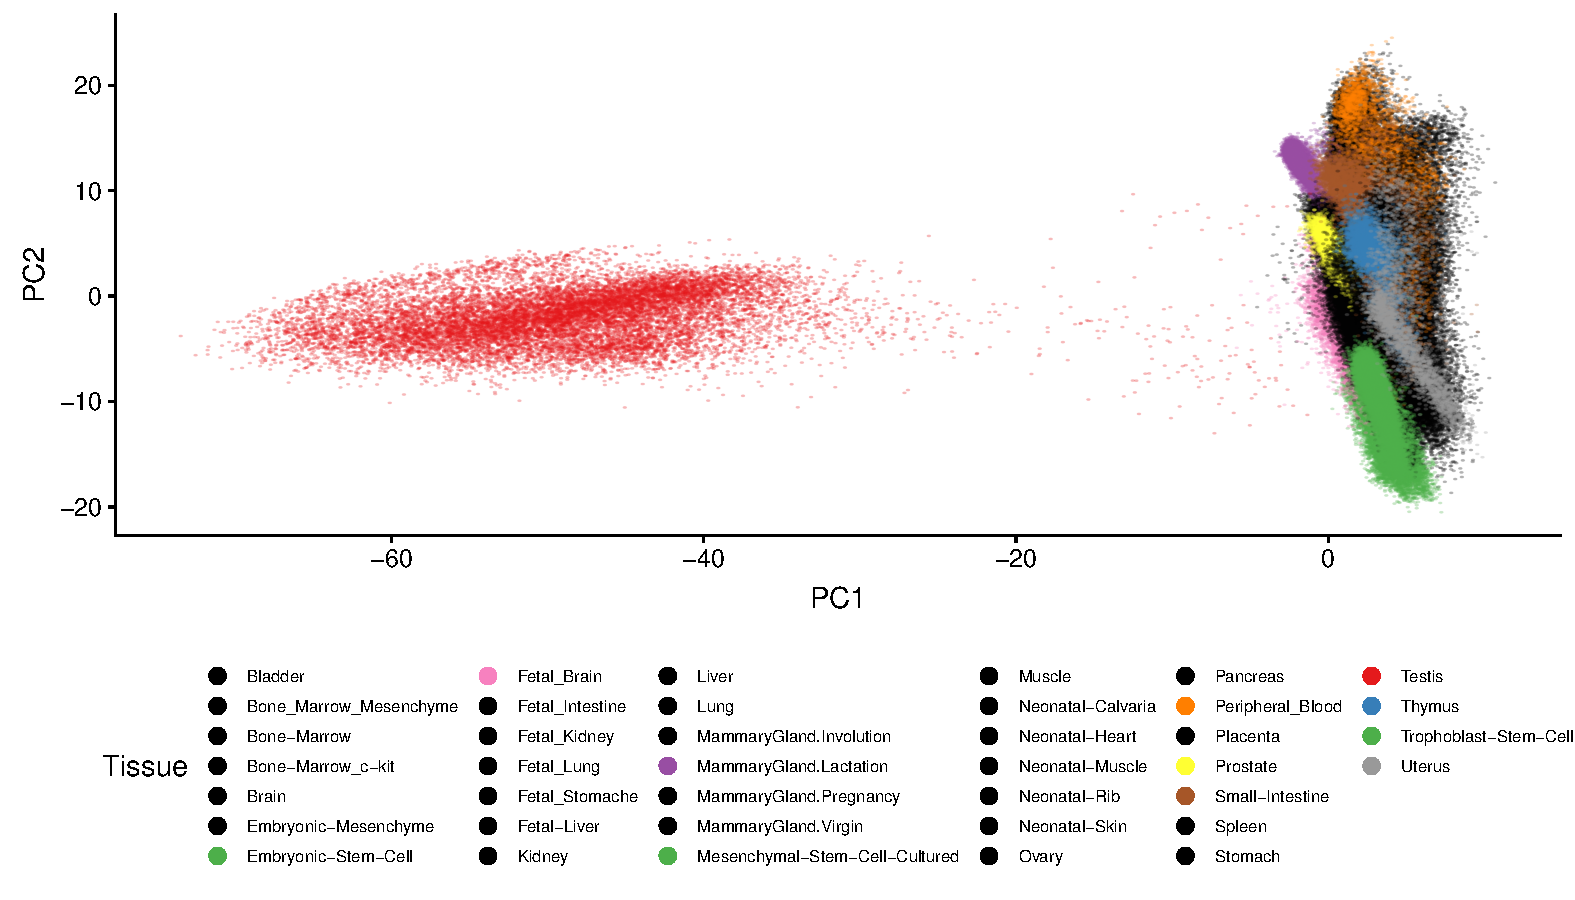
\includegraphics[width=\textwidth]{figures/intro/MCA_PCA.pdf}
	\caption[Testis PCA (MCA)]{PCA of single cell RNAseq of 50 different tissues and cell types from over 400,000 cells from the mouse. Data from~\cite{Han2018Mapping}}
	\label{fig:MCA_PCA}
\end{figure}


 The previous two properties have lead to the use of testis expressed genes as targets for cancer immunotherapy (cancer testis antigens) as when re-expressed in cancers they provide a distinguishing biomarker \parencite{Whitehurst2014Cause}.

Chromatin undergoes massive remodelling during spermatogenesis ultimately resulting in most (90/99\% in human/mouse) of the histones being replaced by crosslinked protamines, leading to the cessation of transcription \parencite{Rathke2014Chromatin}. This necessitates long term mRNA storage ($>$5 days) before translation \parencite{Kleene2013Connecting}.

Sperm are a highly specialised cell, despite being a single cell and unable to transcribe new mRNA they must perform many of the functions of the whole organism including motility, sensing the environment (chemotaxis), and defence from attack (from the female immune system) \parencite{Kaupp2008Mechanisms, Thompson1992Leukocytic}. Indeed they are able to survive and even fertilise after more than three days in the female reproductive tract \parencite{Gould1984Assessment,Wilcox1995Timing}.

Meiosis itself of course is also unique, with paternal and maternal homologous chromosomes being blissfully unaware of each other in somatic cells, until pairing in meiosis in the germline.

%Incomplete cytokinesis


\subsection{Mapping Projects of Science}

Much of science can be characterised as the creation of maps. The discovery, description and cataloguing of various types of elements, which is often dismissed as 'merely descriptive', is a fundamental bedrock of many sciences \cite{Grimaldi2007Why}. Maps are often useful in two senses, they server as a reference of what's already known, but also arrange current knowledge in such a way as to provide a prediction of the unknown. For example Mendeleev's periodic table both catalogued the known elements but left gaps for new discoveries. Equally with the Standard Model in physics. Darwin and others made extensive catalogues of past and present diversity of life, eventually resulting in the concept of evolution by natural selection. Cataloguing the ratios of offspring lead to Mendels laws.

The human genome project provided a single base pair map of our DNA, which not only accelerated research by providing a reference and enabling new bioinformatic analyses, but also uncovered many genes and conserved sequences of unknown function. Other atlases such as the Human Protein Atlas and GTEx which compiled gene expression data went some way to shed light on these genes by associating tissue specific genes with the function those tissues. Now the wave of single cell resolution expression atlases such as the Human Protein Atlas and Mouse Cell Atlas as well as other tissue specific maps including this one, provide even higher resolution clues for the function of unstudied genes of which there are many \parencite{X}.




\section{Gametogenesis}
Gametogenesis is the process by which primordial germ cells develop into either spermatozoa in the male (spermatogenesis) or ovum in the female (oogenesis).

\subsection{Oogenesis}
Whilst equally important to spermatogenesis oogenesis process is studied far less (1,099 vs 359 articles indexed in PubMed 2018). This is likely partially due to difficulties in studying oogenesis compared to spermatogenesis. In oogenesis prophase I up to diplotene occurs in the ovary of the fetus before birth at which point meiosis is arrested (``Dictyate''), making experiments more challenging.

\subsection{Stages of Meiosis}
\subsubsection{Meiosis I}
Meiosis is preceeded by DNA replication much like in mitosis and so initiates from cells that are 2n, 4c (n = ploidy / number of centromeres; c = number of chromosomes).
\subsubsection{Prophase I}
Prophase is much longer in meiosis than mitosis and so is itself split into a number of phases.

During meiosis there is an extended prophase I (lasting 14 days in mice), which is itself divided into a number of stages: Leptotene, Zygotene, Pachytene, and Diplotene. In Leptotene and Zygotene the homologous chromosomes undergo presynaptic pairing, aided by meiosis-specific cohesin, and Spo11 creates several hundred programmed double-strand breaks at sites bound by Prdm9, the only known mammalian speciation gene (Mihola et al., 2009). 


\subsubsection{Leptotene}

\subsubsection{Zygotene}
\subsubsection{Pachytene}
\subsubsection{Diplotene}
\subsubsection{Diakinesis}
\subsubsection{Metaphase I}
\subsubsection{Anaphase I}
\subsubsection{Telophase I}

\subsubsection{Meiosis II}


\subsection{Stages of Spermatogenesis}
In males meiosis takes place during a broader developmental program called spermatogenesis which encompasses the path from spermatogonial stem cells through to maturing spermatozoa. This process it itself supported by a number of somatic cells both within and surrounding the seminiferous tubules.

 Furthermore, testes are a mixture of cells including spermatogonia, which give rise to primary and secondary spermatocytes, which themselves develop into early and late spermatids, Sertoli cells which engulf and nurse the spermatocytes, as well as Leydig (interstitial) cells which secrete androgen hormones~(figure~\ref{fig:histology}). Many of these cells are not meiotic and so the gene expression values from bulk tissue are an average of all these cells and so can not be used to fully delineate gene expression patterns in meiosis itself.

\begin{figure}[H]
	\centering
	\includegraphics[width=\textwidth]{figures/histology.png}
	\caption{Cross section of a seminiferous tubule in testis with the main cell types labelled, reproduced from~\cite{Junqueira2005Basic}}
	\label{fig:histology}
\end{figure}

Other studies have transcriptionally profiled only testis tissue and have tried to target specific meiotic cells. For example the initial wave of spermatogenesis is somewhat synchronous and so sampling during this time could in theory yield homogeneous cell types/stages. However it is likely there is some variation in synchronicity resulting in impure samples and uncertain classification~\cite{Laiho2013Transcriptome,Ball2016Regulatory}. One study utilised the greater synchrony of meiosis in fetal ovaries in combination with germ cell depleted mutant mice to delineate the meiotic prophase gene regulatory programme~\cite{Soh2015Gene}. Other approaches include either size based centrifugal sorting~\cite{Soumillon2013Cellular,Buard2009Distinct,Grabske1975Centrifugal} or FACS (Flourescence Activated Cell Sorting) using a DNA stain~\cite{daCruz2016Transcriptome}, both of which result in a limited number of (possibly quite heterogeneous) cell populations. Immunohistochemistry enables single cell resolution of protein expression but is low throughput~\cite{Djureinovic2014human}. There is one study using single cell transcriptomics however they focus mainly on pre-meiotic foetal development~\cite{Li2017SingleCell}.

%Recent studies have combined this approach with an in silico deconvolution or machine learning algorithms~\cite{Margolin2014Integrated,Li2013Identification}.

Knowledge of the yeast gene regulatory programme of meiosis is relatively well known, however, the lack of sequence similarity and inability to culture mammalian meiotic cells has hampered efforts to translate this network to more complex eukaryotes~\cite{Brar2011HighResolution,Mata2002transcriptional,Chu1998Transcriptional,Handel2010Genetics}.



%%%%%%%%%%%%%%%%%%%%%%%%%%%%%%%%%%%%%%%%%%%%%%%%%%%%%%%%%%%%%%%%%%%%%%%%
\section{Measuring Gene Expression}
%%%%%%%%%%%%%%%%%%%%%%%%%%%%%%%%%%%%%%%%%%%%%%%%%%%%%%%%%%%%%%%%%%%%%%%%

Expression is the process in which information contained in the genome is 
There are a number of different technologies available to quantify the amount of mRNA each providing different information.

\subsection{In Situ Hybridization}
In Situ Hybridisation uses a probe (either RNA or DNA) which is incubated with fixed cells and binds to a target mRNA by complementary binding. 

Radioactive labelling was low resolution, expensive, unstable, and dangerous. but this was overcome by biotinylated probes couples with secondary detection \parencite{Singer1982Actin} and later directly flourescent probes \parencite{Kislauskis1993Isoformspecific}.

This technique has been extended to measure individual mRNA molecules by using multiple probes per target RNA (single molecule smFISH) \parencite{Raj2008Imaging, Femino1998Visualization}. In addition to multiplexed detection to enable many (up to X) RNA targets to be measured at once \parencite{}.


\subsection{RT-qPCR}
Reverse transcription quantitative real-time PCR measures PCR products during the amplification by using fluorescent detectors \parencite{Gibson1996novel, Heid1996Real, Chiang1996Use}. This technique is able to detect a single molecule, however any spatial information is lost.

Due to the exponential amplification, small differences in reverse transcription, primer efficiency, or initial starting amounts and contamination can lead to inaccurate quantification. Therefore, efficiency and validated reference genes must be established by separate experiments \parencite{Bustin2009MIQE}.

\subsection{Northern Blot}
The Northern blot (RNA extraction, separation by gel electrophoresis, followed by transfer by blotting onto a membrane and finally detection by complementary hybridisation with a radioactive/fluorescent probe)  is one of the earliest methods for measuring mRNA levels \parencite{Alwine1977Method}. Northern blotting still remains a useful technique when information about the relative sizes of transcripts is required.

\subsection{Microarrays}


\subsection{Bulk RNAseq}


\subsection{Single Cell RNAseq}


\subsection{Droplet Based Technologies}


\subsection{Extensions}


\section{Statistical Methods}

Although the methods and workflow for analysing bulk RNAseq are now fairly mature and standardised, scRNAseq data has characteristics such as sparsity and high N which are poorly handled by bulk RNAseq tools. In addition scRNAseq data has opened up new analysis possibilities such as pseudotemporal ordering which is not possible with bulk data. This has motivated the development of many (\textgreater 120) new methods and analysis packages to meet the new demands and challenges of analysing scRNAseq data~\cite{Zappia2017scRNAtools}.

The sparse nature and low signal-to-noise ratio of scRNAseq data is partly due to the low number of molecules being measured. For example many transcripts are present at \textless 10 copies per cell, and yet these transcripts could be important given protein to mRNA ratios commonly exceed 1,000~\cite{Lahtvee2017Absolute,Marguerat2012Quantitative}. In addition there is large natural variation in expression between comparable cells due to stochastic bursting gene expression kinetics~\cite{Raj2006Stochastic}. These challenges are compounded by inefficiencies and biases at each step of the library preparation procedure (cell lysis, mRNA capture, reverse-transcription, amplification) resulting in losses of 50 to 90\%~\cite{Islam2012Highly}.

There two major analysis modes for scRNAseq: ordering of cells (in the case of differentiating cells), and clustering of cells into types (either to discover new cell types, or for downstream analysis on each type for example to define the transcriptional profile). However, before this is done dimensionality reduction is often performed on the (log transformed) gene by cell count matrix. Standard Principal Components Analysis (PCA) or Independent Component Analysis (ICA) are popular methods due to their speed and ease of interpretation~\cite{Satija2015Spatial,Trapnell2014dynamics}. Other linear reductions such as Non-Negative Matrix Factorisation (NMF)~\cite{Shao2017Robust} and factor analysis~\cite{Buettner2015Computational} have also been used. Some of these methods have been adapted specifically for single cell analysis, for example ZIFA is a factor analysis which accounts for the sparsity of single cell data by including a zero-inflation component in the model (Zero Inflated Factor Analysis)~\cite{Pierson2015ZIFA}.

Nonlinear dimensionality reduction is also used, especially t-SNE (t-distributed Stochastic Network Embedding), but self organising maps, locally linear embedding, Gaussian process latent variable models, and diffusion maps have also been proposed~\cite{Kim2015SingleCell,Welch2016SLICER,Haghverdi2015Diffusion,Campbell2015Bayesian}.

\begin{figure}[H]
	\centering
	\includegraphics[width=\textwidth]{figures/pseudotime_methods.png}
	\caption{Comparison of pseudotime inference methods, reproduced from~\cite{Cannoodt2016Computational}}
	\label{fig:pseudotime_methods}
\end{figure}

After dimensionality reduction, downstream analysis such as clustering of cells is then achieved using methods such as k-means, hierarchical clustering, density clustering, or consensus clustering~\cite{Zurauskiene2016pcaReduce,Kiselev2017SC3,Guo2015SINCERA,Satija2015Spatial}. Pseudo-temporal ordering of cells is typically achieved by creating a minimum spanning tree and then projecting cells onto the shortest path to create a timeline~\cite{Trapnell2014dynamics,Ji2016TSCAN} (figure~\ref{fig:pseudotime_methods}). Alternatively a principal curve or graph can be used~\cite{Marco2014Bifurcation,Qiu2017Reversed}.


% Similar aims (delineating lineage hierarchies and transcriptional networks) have been achieved using single cell RNA-seq in tissues other than testis, highlighting the feasibility of this study~\cite{Trapnell2014Dynamics,Treutlein2014Reconstructing,DurruthyDurruthy2014Reconstruction,Moignard2013Characterization,Stegle2015Computational}.


\subsection{Principal Components Analysis}

\subsection{Factor Analysis}

\subsection{Sparsity}

%Frequentist
%Bayesian



\section{Prior Work}


Some studies such as GTEx (Genotype-Tissue Expression), HPA (Human Proteome Atlas), and FANTOM (Functional Annotation Of Mammalian genome) consortia have transcriptionally profiled many whole tissues in humans~\cite{Mele2015Human,Uhlen2015Tissuebased,Uhlen2016Transcriptomics}. This data enables the identification of tissue specific genes and hence a preliminary list of proteins which could be involved in meiosis.  However, this could be due to generally pervasive transcription in germ cells due to permissive chromatin~\cite{Soumillon2013Cellular}.



RNA sequencing (RNAseq) has enabled the probing of these mechanisms at a transcriptional level. However, our current knowledge of the meiotic gene expression programme is low resolution. This is partly due to heterogeneity of the cell population in testes which is averaged by bulk tissue RNAseq~\cite{YasuhiroFUJIWAR2014Differential} as well as the relative inability to culture mammalian meiotic cells in vitro~\cite{Zhou2016Complete}. The recent introduction of single cell RNAseq (scRNAseq)~\cite{Gawad2016Singlecell}, raises the possibility of identifying the gene expression profile associated with different stages of meiosis. This may enable the identification of the meiotic transcriptional network as well as aid in the discovery and understanding of meiotic mechanisms.
